\documentclass[main.tex]{subfiles}
\ProvidesPackage{preamble}

\usepackage[nottoc]{tocbibind}
\usepackage[english]{babel}
\usepackage[utf8]{inputenc}
\usepackage[table]{xcolor}
\usepackage[nohead, nomarginpar, margin=1in, foot=.25in]{geometry}
\usepackage{tabularx}
\usepackage{graphicx}
\usepackage{float}
\usepackage[english]{babel}
\usepackage{paralist}
\usepackage{datetime}
\usepackage{afterpage}

\begin{document}

\section{Branding}
We have started the prcess of creating a brand for our product by looking at books and articles on branding. The two most useful resources we have seen are  \cite{basics_branding}, \cite{clifton_2009}. Based on knowledge acquired we have decided that our brand needs a Name,  a Logo, a Motto and an official colour scheme. 
\subsection{Name and Logo}
In order to find a name and a logo that would represent us, we have done a brainstorming session where we have laid out the keywords that represent our product. Out of all the words we listed, two recurring categories of keywords appeared, those were flourishing and data science. We then went on to find ways of representing those. For the flourishing part, we have decided on choosing Thalia as the name of the product. Thalia is a Greek muse often described as the flourishing, the growing one. We saw the association between our product and the Greek muse of growth as a good one given that by using our product the people who invest should also experience flourishing and for the data science part  the Ancient Greeks have a very strong connection to the concept of science. \newline\newline
In order to create a logo to our liking, we have asked a friend skilled in design to create it Pro Bono for us. As a result, we now have a logo that is both representative and that can be legally used.


\begin{figure}[H]
    \centering
    \caption{Logo \cite{TR}}
    
\includegraphics[width=0.5\textwidth]{Pictures/small_logo.png}
\end{figure}


\subsection{Motto}
We have decided that our motto should be something that would reassure our customers that they have made the right choice \cite{motto_creation}. One way of doing this was to make the motto point exactly what our target audience needs. In this case, our target audience wants reliable backtesting. As a result, we have come up with a simple motto, "Thalia the reliable Backtester".



\subsection{Official colours} 
 After consulting some sources on Color theory \cite{how_to_color_palette} we have seen that we should start from choosing the base colour of our palette. In order to be up to date with the latest design trends, we have sought to use something close to the colour of the year 2020 \cite{pantone}. Based on this colour we have created three colour palettes that we could use.

After some deliberation inside the team and some feedback from a few outside people, we have decided to use the third option.      
In the following figure, the final three colour schemes are presented with the chosen one named Thalia and third one looking left to right.

\begin{figure}[H]
    \caption{Color schemes \cite{TR}}
    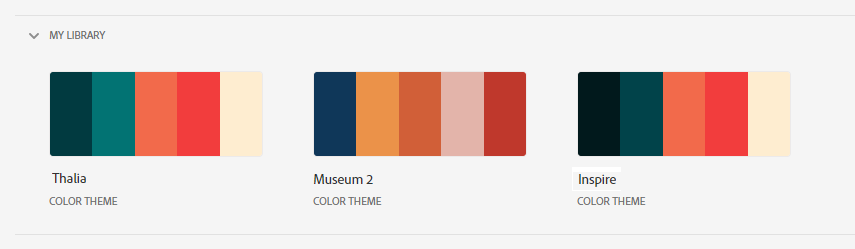
\includegraphics[width=\textwidth]{03Branding/Pictures/color_schemes.png}
\end{figure}


\end{document}    